\documentclass[12pt]{article}
\usepackage[margin=2.5cm]{geometry}
\usepackage{enumerate}
\usepackage{amsfonts}
\usepackage{amsmath}
\usepackage{fancyhdr}
\usepackage{amsmath}
\usepackage{amssymb}
\usepackage{amsthm}
\usepackage{mdframed}
\usepackage{graphicx}
\usepackage{subcaption}
\usepackage{adjustbox}
\usepackage{listings}
\usepackage{xcolor}
\usepackage{booktabs}
\usepackage[utf]{kotex}
\usepackage{hyperref}

\definecolor{codegreen}{rgb}{0,0.6,0}
\definecolor{codegray}{rgb}{0.5,0.5,0.5}
\definecolor{codepurple}{rgb}{0.58,0,0.82}
\definecolor{backcolour}{rgb}{0.95,0.95,0.92}

\lstdefinestyle{mystyle}{
    backgroundcolor=\color{backcolour},
    commentstyle=\color{codegreen},
    keywordstyle=\color{magenta},
    numberstyle=\tiny\color{codegray},
    stringstyle=\color{codepurple},
    basicstyle=\ttfamily\footnotesize,
    breakatwhitespace=false,
    breaklines=true,
    captionpos=b,
    keepspaces=true,
    numbers=left,
    numbersep=5pt,
    showspaces=false,
    showstringspaces=false,
    showtabs=false,
    tabsize=1
}

\lstset{style=mystyle}

\pagestyle{fancy}
\renewcommand{\headrulewidth}{0.4pt}
\lhead{CSC 373}
\rhead{Worksheet 5 Solution}

\begin{document}
\title{CSC373 Worksheet 5 Solution}
\maketitle

\bigskip

\begin{enumerate}[1.]
    \item

    \bigskip

    \underline{\textbf{Notes}}

    \begin{itemize}
        \item \textbf{Maximum Flow Problem:}

        \begin{itemize}
            \item Is about computing the greatest rate at which we can ship material from the source to the sink without
            violating any capacity constraints
        \end{itemize}

        \bigskip

        \item \textbf{Flow Network:}
        \begin{itemize}
            \item $G = (V,E)$ is a directed graph in which each edge $(u,v) \in E$
            has a nonnegative capacity $c(u,v) \geq 0$.
            \item Two vertices must exist: \textbf{source} s and \textbf{sink} t
            \item \textbf{path} from source $s$ to vertax $v$ to sink $t$ is represented by $s \rightsquigarrow v \rightsquigarrow t$

        \end{itemize}

        \bigskip

        \begin{center}
        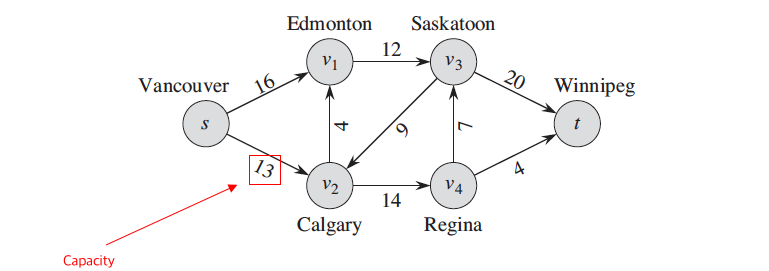
\includegraphics[width=0.9\linewidth]{images/worksheet_5_solution_1.png}
        \end{center}

        \item \textbf{Capacity:}

        \begin{itemize}
            \item
        \end{itemize}

        \item \textbf{Flow:}


    \end{itemize}

\end{enumerate}

\end{document}